
%% Version 0.3

%%%%%%%%%%%%%%%%%%%%%%%%%%%%%%%%%%%%%%%%%%%%%%%%%
%%                                             %%
%%   This LaTeX template is intended for       %%
%%   use with IEEE Computer Society Magazines  %%
%%   as an alternative to the MS Word          %%
%%   template.                                 %%
%%                                             %%
%%%%%%%%%%%%%%%%%%%%%%%%%%%%%%%%%%%%%%%%%%%%%%%%%


\documentclass{csmagazine}

\usepackage{listings}


%%%%%%%%%%%%%%%%%%%%%%%%%%%%%%%%%%%%%%%%%%%%%%

%OPTIONAL: Declare unicode characters that are not easily created by single LaTeX commands

%Example of delcaring a special character to use later in the document
\DeclareUnicodeCharacter{1EBF}{\'{\^{e}}}


%%%%%%%%%%%%%%%%%%%%%%%%%%%%%%%%%%%%%%%%%%%%%%


%%%%%%%%%%%%%%%%%%%%%%%%%%%%%%%%%%%%%%%%%%%%%%
%%                                          %%
%% Enter the title of your article below    %%
%%                                          %%
%%%%%%%%%%%%%%%%%%%%%%%%%%%%%%%%%%%%%%%%%%%%%%


\title{A Guide to Using the IEEE Computer Society LaTeX Template for Magazines.}


%%%%%%%%%%%%%%%%%%%%%%%%%%%%%%%%%%%%%%%%%%%%%%
%%                                          %%
%% Enter the authors of your article below. %%
%% Put a line break \\ after each author    %%
%% use \ieeecsAffiliaiton{} after the       %%
%% author name to assign an affiliation     %%                
%% use \ieeecsnoAffiliation if the author   %%
%% has no affliation, to create appropiate  %%
%% spacing                                  %%
%%                                          %%
%%%%%%%%%%%%%%%%%%%%%%%%%%%%%%%%%%%%%%%%%%%%%%


\author{%
	First Author\\ \ieeecsAffiliation{First Author Affiliation}\\
	Second Author\\	\ieeecsnoAffiliation
	Third Author\\ \ieeecsAffiliation{Third Author Affiliation}\\ 
}


%%%%%%%%%%%%%%%%%%%%%%%%%%%%%%%%%%%%%%%%%%%%%%
%%                                          %%
%% Update the page headers below with the   %%
%% section name and magazine title your     %%
%% article will appear in.                  %%
%%                                          %%
%%  Section title = The Title of the        %%
%%  section this article will appear in.    %%
%%  Found in EMS.                           %%
%%                                          %%
%%  MAGAZINE TITLE = The magazine name you  %%
%%  are writing for                         %%
%%%%%%%%%%%%%%%%%%%%%%%%%%%%%%%%%%%%%%%%%%%%%%


%include your bib file here
\addbibresource{refs.bib}


\begin{document}	


\ieeecsPageHeaders{The Title of the Section the Article Belongs To}{TITLE OF THE MAGAZINE}

\ieeecsArticleTitle


\ieeecsInsertAuthor


%%%%%%%%%%%%%%%%%%%%%%%%%%%%%%%%%%%%%%%%%%%%%%
%%                                          %%
%% The abstract goes here                   %%
%%                                          %%
%%                                          %%
%%%%%%%%%%%%%%%%%%%%%%%%%%%%%%%%%%%%%%%%%%%%%%


\ieeecsAbstract{This template (cs.tex) is meant to provide authors of IEEE Computer Society magazine articles a guide to preparing your article in LaTeX for submission, as well as to be used as a starting point that you can edit with the contents of your paper. This is a sample abstract. Abstracts should be single paragraphs that cannot contain math or citations. Please use the \textbf{\textbackslash{}ieeecsAbstract\{\}} command for abstracts. If your paper does not contain an abstract please remove this command and instead un-comment the \textbf{\textbackslash{}ieeecsNoAbstract} command to apply the correct formatting. The abstract will appear in a sans-serif font.}

%%%%%%%%%%%%%%%%%%%%%%%%%%%%%%%%%%%%%%%%%%%%%%
%%                                          %%
%%											%%
%% If your paper has no abstract, remove    %%
%% the \ieeecsAbstract command above and    %%
%% un-comment the \ieeecsNoAbstract command	%%
%% below.									%%
%%                                          %%
%%%%%%%%%%%%%%%%%%%%%%%%%%%%%%%%%%%%%%%%%%%%%%



%\ieeecsNoAbstract



%%%%%%%%%%%%%%%%%%%%%%%%%%%%%%%%%%%%%%%%%%%%%%
%%                                          %%
%% The introduction starts below            %%
%% You may have several intro. 				%%
%% paragraphs each using the 				%%
%% \ieeecsIntroduction command              %%
%%                                          %%
%%%%%%%%%%%%%%%%%%%%%%%%%%%%%%%%%%%%%%%%%%%%%%


Insert your introduction here. Your introduction can be one or more paragraphs and will appear before any main sections. The introduction does not need a section heading and should be no longer than three paragraphs. It may contain math and citations. There is no special command needed for introductions, it can created by paragraphs of text that appear before the first \textbf{\textbackslash{}section command}.

\section{Sections and the Body of the Article}

The body of an article is broken into sections. Up to three section levels are supported using \textbf{\textbackslash{}section\{Title\}}, \textbf{\textbackslash{}subsection\{Title\}}, and \textbf{\textbackslash{}subsubsection\{Title\}}. Avoid "lone" headings, for example, a level-2 head without another level-2 head in the same section. Also avoid "stacked" headings. Two or more consecutive headings must be separated by intervening text (even if it's just a sentence or two).

\subsection{Formatting text}

Simple paragraphs can be entered without any additional LaTeX commands. For italic text please use the \textbackslash{}textit\{\} command \textit{italic text example}. For bold text please use the \textbackslash{}textbf\{\} command \textbf{bold text example}. For underlined text please use the \textbackslash{}underline\{\} command \underline{underlined text example}.

URLs can be created using the \textbackslash{}url\{\} command for example: \url{https://www.computer.org} command.

To enter text that retains formatting, such as program code, please use the verbatim environment.

\begin{verbatim}
1. Example of using verbatim for writing algorithms
2. It can also be used for small blocks of code
3. Text within it can be further styled such as /emph{italic text} 
...
4. End.
\end{verbatim}


\begin{lstlisting}[language=PhP]
$articleBaseName = basename($articleTeXFile, ".tex");
$articleXMLFile = basename($articleTeXFile, ".tex");
\end{lstlisting}

\subsubsection{Special characters}

To insert "Special characters" (symbols other than the lowercase letters a–z, uppercase letters A-Z, numbers 0–9, and English punctuation marks) that are not easily created with a single LaTeX command such as \textbackslash{}'\{a\} please use one of the the following options.

Option 1: Insert the glyph of the character within the \textbf{\textbackslash{}\{fontencoding\{EN\}\textbackslash{}selectfont X\}} command where EN is the encoding to use and X is the glyph to output.

% example of using \fontencoding to select T5 econding to display the ế character
%{\fontencoding{T5}\selectfont ế} 

Option 2: Delcare the character with \textbf{\textbackslash{}DeclareUnicodeCharacter\{character code\}\{LaTeX command\}} in the preamble. You can then use that character with your text withou additional commands. Example: ế.

% Commands for common accented characters (the letter x is used for example)

% \`{x} %grave accent
% \'{x} %acute accent
% \^{x} %circumflex
% \"{x} %umlaut, trema or dieresis
% \H{x} %long Hungarian umlaut (double acute)
% \~{x} %tilde
% \c{x} %cedilla
% \k{x} %ogonek
% \l{} %barred l
% \={x} %macron accent
% \b{x} %bar under the letter
% \.{x} %dot over the letter
% \d{x} %dot under the letter
% \r{x} %ring over the letter (for å there is also the special command \aa)
% \u{x} %breve over the letter
% \v{x} %caron over the letter
% \t{xx} %tie (inverted u) over the two letters
% \o %o with stroke)


\subsection{Math}

For numbered display equations, please use the \textbf{equation} environment. For display equations that should not be numbered please use the commands \textbackslash[...\textbackslash]. Please use these commands for display math instead of the double dollar signs `\$\$'.

\textbf{Example of a numbered display equation:}

%Example of a numbered display equation. Please use \begin{equation} for numbered display math
\begin{equation}
\sqrt{\frac{x^2}{k+1}}\qquad
x^\frac{2}{k+1}\qquad
\frac{\partial^2f}{\partial x^2}
\end{equation}

\textbf{Example of an un-numbered display equation:}

%Example of an un-numbered display equation. Please use \[...\] instead of $$...$$ for un-numbered display math
\[\binom{n}{k} =\binom{n-1}{k} + \binom{n-1}{k-1}\]


For inline math please use the single `\$' symbols. Example of inline math: $\int\frac{d\theta} {1+\theta^2}=\tan^{-1} \theta+C$.

\subsection{Lists}

\textbf{A bulleted list}

%Example of a bulleted list
\begin{itemize}
	\item First item
	\item Second item
	\item Third item
	\item Fourth item
\end{itemize}

\textbf{A Numbered List}

%Example of a numbred list
\begin{enumerate}
	\item The labels consists of sequential numbers.
	\item The numbers starts at 1 with every call to the enumerate environment.
\end{enumerate}




%%%%%%%%%%%%%%%%%%%%%%%%%%%%%%%%%%%%%%%%%%%%%%
%%                                          %%
%% Sections Begin Here                      %%
%%                                          %%
%%                                          %%
%%%%%%%%%%%%%%%%%%%%%%%%%%%%%%%%%%%%%%%%%%%%%%


\section{Figures and Tables}

When submitting your paper, please be sure include all graphics reference by your source file. File formats allow for graphics are as follows: \textbf{PDF, PNG, JPEG, \& EPS}.

\subsection{Figures}

Figures should be created as a single graphic per figure. We cannot support multiple graphics as seperate parts of the same figure, or using LaTeX pagackages to draw graphics. Each figure should contain a caption. If you have created a figure as mulitple parts please combine them first as a single graphic before references the graphic from this template.

%%%%%%%%%%%%%%%%%%%%%%%%%%%%%%%%%%%
%%                               %%
%% Figure example                %%
%%                               %%
%%  All graphics must be         %%
%% submitted separately and not  %%
%% included in the Tex document  %%
%%                               %%
%% Figures need be created as    %%
%% a single image per figure and %%
%% where all parts 'a', 'b',     %%
%% etc. are included in one      %%
%% image.                        %%
%%                               %%
%%                               %%
%%%%%%%%%%%%%%%%%%%%%%%%%%%%%%%%%%%

\begin{figure}[H]
	\begin{center}	
		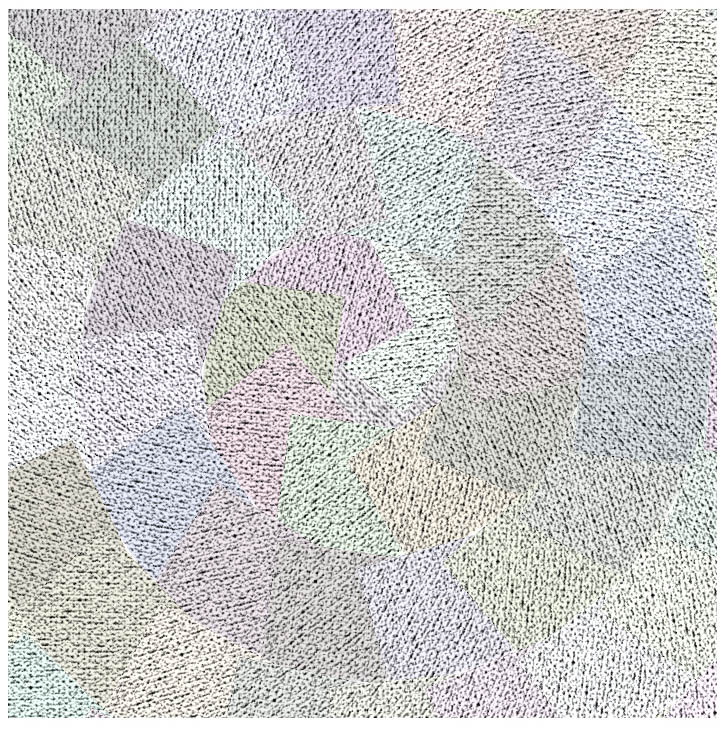
\includegraphics[width=0.5\textwidth]{figure_1.jpg}
		\caption{Add your figure caption Here \label{fig:example_fig}}		
	\end{center}
\end{figure}


You can reference a figure using the \textbackslash{}ref\{\}command. Example: see figure \ref{fig:example_fig}. Be sure that the \textbackslash{}label\{\} command is inside of the \textbackslash{}\{\}caption command for for your figure for the numbering to be correct. Below is an example of a second figure, using an EPS file as the graphic.


\begin{figure}[H]
	\begin{center}	
		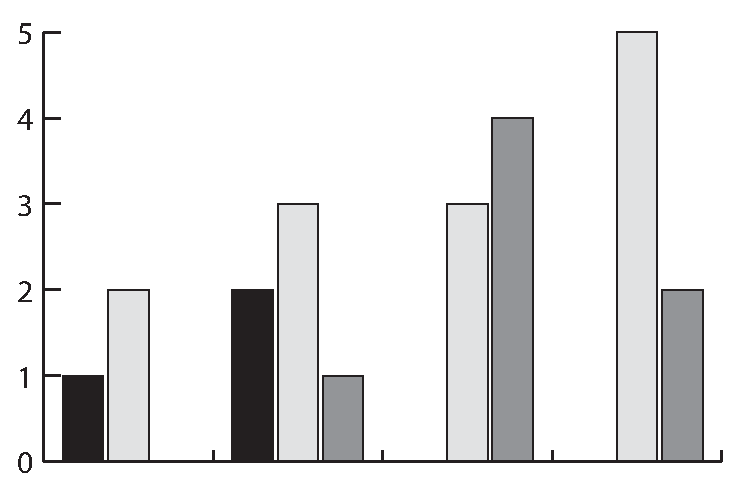
\includegraphics[width=0.5\textwidth]{figure_2.eps}
		\caption{Add your figure caption Here \label{fig:example_fig2}}		
	\end{center}
\end{figure}

To include graphics in your article that should not be considerd a figure, and should not have a caption or label, please use the \textbackslash{}includegraphics\{\} command.

Example of a graphic that is not a figure:

\includegraphics[width=0.25\textwidth]{graphic_1.png}

\subsection{Tables}

Tables can be created in one of two ways. You can use the tabluar environment to build your table within LaTeX, or you can reference a graphic that you have created outside of LaTeX to represent your table. Tables require a title added using the custom \textbackslash{}ieeecsTableTitle\{\}



%%%%%%%%%%%%%%%%%%%%%%%%%%%%%%%%%%%
%%                               %%
%% Table examples                %%
%%                               %%
%%%%%%%%%%%%%%%%%%%%%%%%%%%%%%%%%%%

\begin{table}[H]
	\begin{center}
		\ieeecsTableTitle{A table created in LaTeX using tabular}
		\begin{tabular}{ |c|c|c|c| } 
			\hline
			col1 & col2 & col3 \\
			\hline
			\multirow{3}{4em}{Multiple row} & cell2 & cell3 \\ 
			& cell5 & cell6 \\ 
			& cell8 & cell9 \\ 
			\hline
		\end{tabular}
	\end{center}
\end{table}


\begin{table}[H]
	\begin{center}
		\ieeecsTableTitle{A table represented by a graphic}
		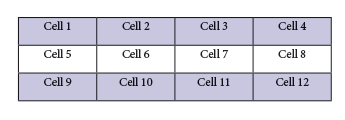
\includegraphics[width=0.5\textwidth]{table_2.png}
	\end{center}
\end{table}

\section{Other Article Elements}

\subsection{Boxed Text}

\fbox{\begin{minipage}{\textwidth - 3em}
Lorem ipsum dolor sit amet, consectetur adipiscing elit. Aenean ut neque ac justo blandit commodo nec aliquam metus. Ut blandit consectetur tincidunt. Fusce quis tellus ex. Ut mattis leo risus. Sed auctor magna id purus sodales dictum in non elit. Aliquam maximus egestas libero in porta. Suspendisse ultricies massa quis sem pellentesque, eu aliquet elit gravida. Ut sagittis eu quam iaculis mattis.
\end{minipage}}

\subsection{Theorems}

...

\subsection{Proofs}

...


\subsection{Program Code}

\lstset{numbers=left, numberstyle=\small, stepnumber=1, numbersep=1em}
\begin{lstlisting}[language=Python]
import numpy as np

def incmatrix(genl1,genl2):
m = len(genl1)
n = len(genl2)
M = None #to become the incidence matrix
VT = np.zeros((n*m,1), int)  #dummy variable

#compute the bitwise xor matrix
M1 = bitxormatrix(genl1)
M2 = np.triu(bitxormatrix(genl2),1) 

for i in range(m-1):
for j in range(i+1, m):
[r,c] = np.where(M2 == M1[i,j])
for k in range(len(r)):
VT[(i)*n + r[k]] = 1;
VT[(i)*n + c[k]] = 1;
VT[(j)*n + r[k]] = 1;
VT[(j)*n + c[k]] = 1;

if M is None:
M = np.copy(VT)
else:
M = np.concatenate((M, VT), 1)

VT = np.zeros((n*m,1), int)

return M
\end{lstlisting}



\subsection{Text between two rules}

\noindent\rule{\textwidth}{1pt}
Lorem ipsum dolor sit amet, consectetur adipiscing elit.
\noindent\rule{\textwidth}{1pt}




\subsection{Logos}

\AllTeX ~ \BibLaTeX

\section{References, Acknowledgements, and Author Bios}

Here is an example of using a citation \cscite{Lamport1994a}.

Another citation \cscite{Goossens1997}.


Lorem ipsum dolor sit amet, consectetur adipiscing elit. Aenean ut neque ac justo blandit commodo nec aliquam metus. Ut blandit consectetur tincidunt. Fusce quis tellus ex. Ut mattis leo risus. Sed auctor magna id purus sodales dictum in non elit. Aliquam maximus egestas libero in porta. Suspendisse ultricies massa quis sem pellentesque, eu aliquet elit gravida. Ut sagittis eu quam iaculis mattis.




%%%%%%%%%%%%%%%%%%%%%%%%%%%%%%%%%%%%%%%%%%%%%%%%%%%%%%%%%%%%%
%%                  The Bibliography                       %%
%%                                                         %%
%%                                                         %%
%%%%%%%%%%%%%%%%%%%%%%%%%%%%%%%%%%%%%%%%%%%%%%%%%%%%%%%%%%%%%

\ieeecsReferences{REFERENCES}

\printbibliography[heading=none]



%%%%%%%%%%%%%%%%%%%%%%%%%%%%%%%%%%%%%%%%%%%%%%%%%%%%%%%%%%%%%
%%                  Acknowledgments                        %%
%%                                                         %%
%%                                                         %%
%%%%%%%%%%%%%%%%%%%%%%%%%%%%%%%%%%%%%%%%%%%%%%%%%%%%%%%%%%%%%

\ieeecsAcknowledgementsHeader{Acknowledgements}

\ieeecsAcknowlegememt{Enter an acknowledgement here.}



%%%%%%%%%%%%%%%%%%%%%%%%%%%%%%%%%%%%%%%%%%%%%%%%%%%%%%%%%%%%%
%%                  Author Bios                            %%
%%                                                         %%
%%                                                         %%
%%%%%%%%%%%%%%%%%%%%%%%%%%%%%%%%%%%%%%%%%%%%%%%%%%%%%%%%%%%%%


\ieeecsAboutAuthor{ABOUT THE AUTHORS}

\ieeecsAuthorBio{Author Name Here}{Author Bio Goes here. Lorem ipsum dolor sit amet, consectetur adipiscing elit. Aenean ut neque ac justo blandit commodo nec aliquam metus. Ut blandit ceonsectetur tincidunt.}

\ieeecsAuthorBio{Author Name Here}{Author Bio Goes here. Lorem ipsum dolor sit amet, consectetur adipiscing elit. Aenean ut neque ac justo blandit commodo nec aliquam metus. Ut blandit consectetur tincidunt.}

\ieeecsAuthorBio{Author Name Here}{Author Bio Goes here.}


\end{document}